\subsection{Achieving generalization}

\textcolor{red}{Talk about image augmentation and show the results}
The intuition that led to finding a viable solution to this hindering issue, is
that the semi-synthetic images are too sharp and do not mirror the amount of
blur seen on real images captured from the UAV in flight.\\

To verify this hypothesis, an image augmentation pipeline was added to the
batch loading process of the network training. In essence, every new batch of
data samples goes through randomized image transformations, ranging from
channel shift and gamma contrast shuffling to additive gaussian noise and
simulated motion blur. Those transformations do not happen in a sequence for
each image of the batch, but rather have different chances of being applied.

The result is a dataset that is augmented differently at every iteration of the
training, thus theoretically introducing an infinite amount of image
variations.

\begin{figure}[h]
	\centering
	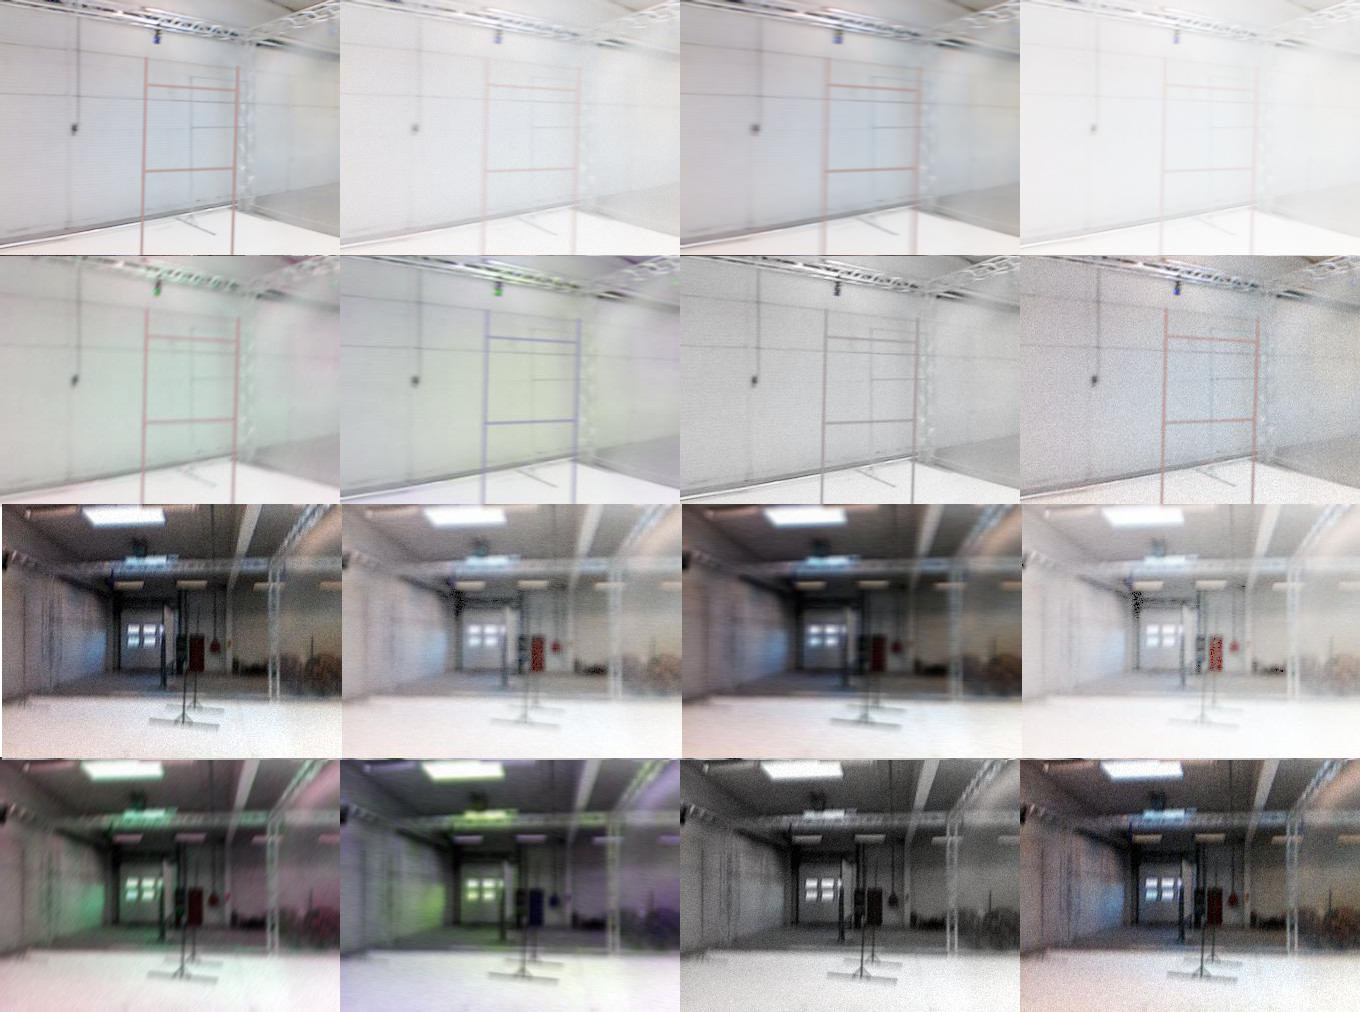
\includegraphics[width=\textwidth]{figure/augmentation.jpg}
	\caption{Few samples of random image transformations applied to one batch.}
	\label{fig:augmentation}
\end{figure}

The effect of applying the said augmentations to the dataset can be seen on
figure~\ref{plot:mobilenetv2-aug}, where each plot compares the augmentation
results to their base counterpart.

\begin{figure}[h!]
	\centering
	\begin{subfigure}{0.49\textwidth}
		\begin{tikzpicture}
			\pgfplotsset{
				scale only axis,
				legend pos=north east,
				legend entries={No augmentation,Augmentation},
				grid style={dotted,gray,line width=.1pt},
				grid=both
			}
			\begin{axis}[xlabel=Epoch,ylabel=Validation loss,width=7cm,height=7cm]
				\addplot+[mark=none,smooth] table [y=val_loss,col sep=comma]
				{plots/mobilenetv2/mobilenetv2_rgb_hidden_dropout_50000.txt};
				\addplot+[mark=none,smooth] table [y=val_loss,col sep=comma]
				{plots/mobilenetv2/mobilenetv2_rgb_hidden_dropout_aug_50000.txt};
			\end{axis}
		\end{tikzpicture}
		\caption{MobileNetV2 with a hidden layer and dropout on 50,000 samples.}
	\end{subfigure}
	\begin{subfigure}{0.49\textwidth}
		\begin{tikzpicture}
			\pgfplotsset{
				scale only axis,
				legend pos=north east,
				legend entries={No augmentation,Augmentation},
				grid style={dotted,gray,line width=.1pt},
				grid=both
			}
			\begin{axis}[xlabel=Epoch,ylabel=Validation loss,width=7cm,height=7cm]
				\addplot+[mark=none,smooth] table [y=val_loss,col sep=comma]
				{plots/mobilenetv2/mobilenetv2_rgb_avg_pooling_50000.txt};
				\addplot+[mark=none,smooth] table [y=val_loss,col sep=comma]
				{plots/mobilenetv2/mobilenetv2_rgb_avg_pooling_aug_50000.txt};
			\end{axis}
		\end{tikzpicture}
		\caption{MobileNetV2 with average pooling on 50,000 samples.}
	\end{subfigure}

	\begin{subfigure}{0.49\textwidth}
		\begin{tikzpicture}
			\pgfplotsset{
				scale only axis,
				legend pos=north east,
				legend entries={No augmentation,Augmentation},
				grid style={dotted,gray,line width=.1pt},
				grid=both
			}
			\begin{axis}[xlabel=Epoch,ylabel=Validation loss,width=7cm,height=7cm]
				\addplot+[mark=none,smooth] table [y=val_loss,col sep=comma]
				{plots/mobilenetv2/mobilenetv2_rgb_hidden_dropout_avg_pooling_noaug_150000.txt};
				\addplot+[mark=none,smooth] table [y=val_loss,col sep=comma]
				{plots/mobilenetv2/mobilenetv2_rgb_hidden_dropout_avg_pooling_aug_150000.txt};
			\end{axis}
		\end{tikzpicture}
		\caption{MobileNetV2 with a hidden layer, dropout and average pooling
		on 150,000 samples.}
	\end{subfigure}
	\begin{subfigure}{0.49\textwidth}
		\begin{tikzpicture}
			\pgfplotsset{
				scale only axis,
				legend pos=south east,
				legend entries={No augmentation,Augmentation},
				grid style={dotted,gray,line width=.1pt},
				grid=both
			}
			\begin{axis}[xlabel=Epoch,ylabel=Validation accuracy,width=7cm,height=7cm]
				\addplot+[mark=none,smooth] table [y=val_accuracy,col sep=comma]
				{plots/mobilenetv2/mobilenetv2_rgb_hidden_dropout_avg_pooling_noaug_150000.txt};
				\addplot+[mark=none,smooth] table [y=val_accuracy,col sep=comma]
				{plots/mobilenetv2/mobilenetv2_rgb_hidden_dropout_avg_pooling_aug_150000.txt};
			\end{axis}
		\end{tikzpicture}
		\caption{MobileNetV2 with a hidden layer, dropout and average pooling
		on 150,000 samples.}
		\label{plot:mobilenetv2-aug-val-large}
	\end{subfigure}
	\caption{Comparison of MobileNetV2 trained on augmented and original
	datasets.}
	\label{plot:mobilenetv2-aug}
\end{figure}


\textcolor{red}{Present top-n accuracies with augmentation.}
